\section{Implementation}
The following sections detail the differences that came about when porting the reference implementation \cite{rainbowgit} to a platform without an operating system, minimal standard library, and more constrained on memory. It will also detail some of the specifics that the original authors used to implement the functionality of Rainbow for reference in later sections. It will, however, not go into detail on how the optimizations tested differ from the original code, see \cref{opti} for this.
\medskip\\
The files and functionality gone through in this section are what is left from porting the implementation to RISC-V. If any changes were made to a file or functionality from the original code it will be described in of the following subsections.
\subsection{Overview of the Reference System}
In general, this port of the Rainbow reference implementation tries to stay as close to its roots as possible, making it easier to argue for correctness and easier to port these findings to other platforms as well (having multiple sources being somewhat similar).
\medskip\\
The variant worked on for this project is solely the standard Rainbow variant with no key-size adjustments and a security level of I. Focusing on this particular variant of the Rainbow scheme makes the optimizations done clearer for readers new to the Rainbow scheme in general, as it is the closest to how Rainbow is described in many sources on Rainbow and the $MQ$ problem and therefore should be somewhat easier than also having to understand some of the key-size reductions going on in \texttt{CZ-Rainbow} and \texttt{Compressed-Rainbow}.
\subsubsection{File Overview}
The files of the reference implementation can be divided into different parts according to what aspect of the Rainbow scheme they partake in. In total, we give an overview of the functionality of this Rainbow port by dividing into these parts and explaining each part separately. First we give an overview of the files in \texttt{src/Ia\_Classic\_Reference}.
\medskip\\
One set of files of this port that had to have quite a lot of changes made to it was the files prepended with \texttt{utils}. These file are to a varying degree part of the internal structure of Rainbow. These files handle random number generation, hashing and $host\rightarrow client$ communication. The hashing aspect of this set is mostly just an API-wrapper for another hashing utility located in \texttt{src/libcrypto}. The changes made to this set of files, and the reasonings, can be seen in \cref{utils}.
\medskip\\
Another set of files is the set consisting of \texttt{rng.c}, \texttt{rng.h}, \texttt{api.h} and \texttt{sign.c}. These files provide NIST-compliance as the NIST standardization requires participating schemes to provide certain functions as an API \cite{nistapi}. These files have not been changed and the output of this project should therefore still be compliant with the NIST standardization API requirements. See \cref{deepdive} for a walkthrough if this API.
\medskip\\
Remaining are two sets of files in \texttt{src/Ia\_Classic\_Reference}, the \texttt{rainbow} files and the library files. The \texttt{rainbow} files consist of all files where \texttt{rainbow} is in the name. These files construct the actual inner-workings of Rainbow and therefore quite well represent how Rainbow works. That is, they make use of all the other files in \texttt{src/Ia\_Classic\_Reference} to provide a simple API to the outermost \emph{tool}-files (more on those later).
\medskip\\
The last set of files in \texttt{src/Ia\_Classic\_Reference} is, as already stated, the library files. These remaining files contain code to run the, mostly, mathematical aspects of the Rainbow scheme. As can be seen in \cref{deepdive}, Rainbow relies on linear algebra and finite field arithmetic. The linear algebra implementations like Guassian elimination, matrix-vector products, vector-vector products, etc. are implemented with finite field arithmetic and therefore all rely on some of the functionality given in \texttt{gf16.h}.
\medskip\\
Moving one directory back, to \texttt{src/}, it becomes clear that most of the Rainbow scheme is implemented in \texttt{src/Ia\_Classic\_Reference}. The only two sets of files of interest are the files prepended with \texttt{rainbow-} and the files in \texttt{src/libcrypto}. The files in \texttt{src/libcrypto} are \texttt{archive} and \texttt{header} files, of an AES and SHA256 implementation, meant for use in some of the files in \texttt{src/Ia\_Classic\_Reference}. The reasoning behind having these files is given in \cref{utils}.\medskip\\
At last are the files \texttt{src/rainbow-*}. These files provide the three different top-level functionalities of rainbow, namely generating keypairs, signing and verifying messages. Should this be a more cohesive construction of rainbow, then one might make a tool that combines these three files into one providing an executable that can seamlessly switch between the functions on-chip instead of having to flash the ROM each time. Though, this might force the ROM usage to be larger than the \texttt{512kB} already specified.
\subsubsection{Utilities} \label{utils}
Due to the constrained nature of an embedded device and/or FPGA, not all the original functionality provided by the Rainbow authors was needed. In particular, dynamic memory allocation was removed entirely due to the somewhat unstable state of using standard library dynamic memory allocation on embedded devices. Instead, all memory allocations are handled by static memory allocation. Alternatively, one could have implemented a sufficient and secure \texttt{malloc} implementation, though this was not deemed necessary for this project.
\medskip\\
The original Rainbow reference implementation also relied on having all data stored in files. As the device running this port of Rainbow has only \texttt{512kB} of ROM and RAM (each), this was changed. This port of Rainbow relies on a host machine connecting to the embedded device and providing signatures, keys, messages and seeds for (cryptographically secure) randomness.
\medskip\\
Although the above two aspects have been altered, they were not aspects that the Rainbow scheme internally was heavily reliant on. Instead, a generally important aspect of Rainbow is the hashing and AES functionality, originally obtained from the OpenSSL library. As the OpenSSL library is quite large, extensive and has no port for the RISC platform that this project is working on some tweaks needed to be made.
\medskip\\
The aspects of OpenSSL used originally by the Rainbow authors were the AES and SHA implementations. The rainbow reference implementation uses either of three SHA-2 variants according to the Rainbow security level \cite{rainbownist}. As this project only focuses on Level I Rainbow, a replacement was needed for the SHA-256 algorithm. The replacement for both the SHA256 implementation and the AES implementation were ones that are used in the official RISC-V github repositories for testing the RISC-V scalar cryptographic instruction set extension proposals currently being examined \cite{riscvcrypt}. These had reference implementations where no special RISC-V instructions were needed, and as such were good candidates for benchmarking on a \textit{reference} system.

\subsection{Deep Dive into Reference Functionality} \label{deepdive}
For this subsection we will be taking a look at what the NIST API enforces, how key generation is actually implemented, how exactly it is that this implementation evaluates the public map on some input and how it signs a document using the inverted maps.
\subsubsection{NIST API}
For public-key signatures, NIST specifies an API consisting of two files and some functionality regarding randomness. The first file specified by NIST is the \texttt{api.h} file. This file lies in the \texttt{src/Ia\_Classic\_Reference} folder and specifies the size of the secret- and public-key, the algorithm name and the byte-overhead allowed for the signed message (how many additional bytes might it take).
\medskip\\
The second file is the \texttt{sign.c} file consisting of \texttt{crypto\_sign()}, \texttt{crypto\_sign\_open()} and \texttt{crypto\_sign\_keypair()} each of which runs a certain aspect of the Rainbow scheme. Respectively, this file consist of the signing mechanism, the verification mechanism and the key-generation mechanism. The functions are also exactly following the NIST-specified declarations.
\medskip\\
The last file is also a pair of header and \texttt{C}-file. These are the \texttt{rng.c} and \texttt{rng.h} files. These files consist of definitions and declarations for \texttt{randombytes()}, \texttt{randombytes\_init()}, \texttt{seedexpander()}, \texttt{seedexpander\_init()} and \texttt{struct AES\_XOF\_struct}. The only thing reworked for this was the AES implementation used for the seed expansion function.
\subsubsection{Key Generation} \label{section:keygen}
The reference key generation of the Rainbow scheme follows \cref{rainbowkeygen}
\begin{figure}[t]
    \centering
    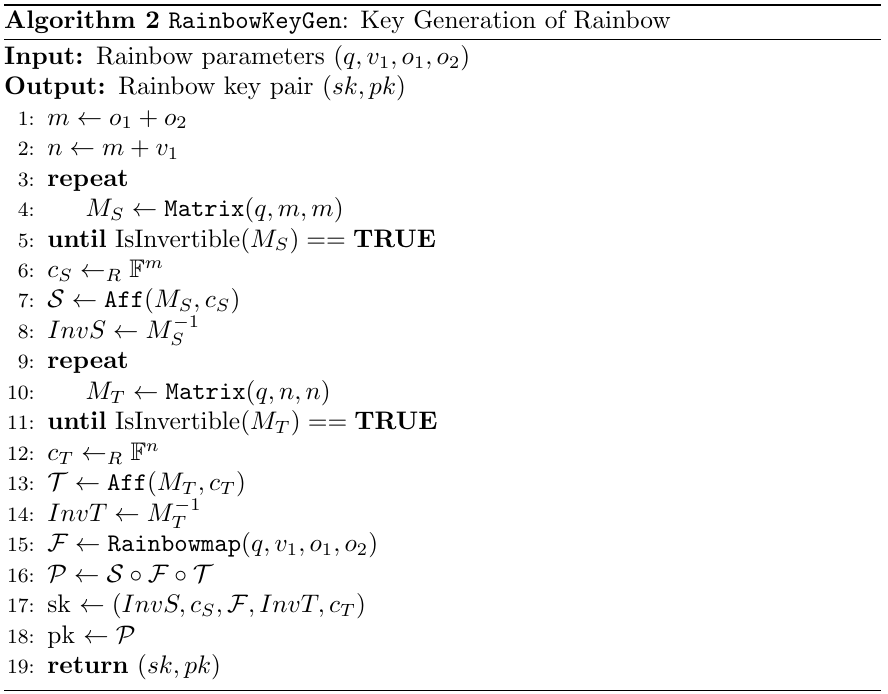
\includegraphics[width=\textwidth]{resources/rainbowkeygen.png}
    \caption{Pseudo code for the Rainbow key generation scheme.}
    \label{rainbowkeygen}
\end{figure}
As this sections has focus on the actual \texttt{C}-implementation of the reference Rainbow scheme, I will bridge the gap between this figure and what is found in the \texttt{Ia\_Classic\_Reference} folder.\medskip\\
Looking at \cref{rainbowkeygen} and making a coupling to \cref{rainscheme} one might clearly see the initialization of important aspects of the key, such as the affine invertible maps $S$ and $T$ generated as $M_S$ and $M_T$ respectively. This initialization is done in lines 3-14 in \cref{rainbowkeygen} whilst line 15 and onward is generation of the central map and at last the generation of the public and secret keys $pk$ and $sk$. The highest-level abstraction of this procedure lies in the \texttt{rainbow\_keypair.c} in \texttt{generate\_keypair()}. This functions is called from the \texttt{NIST}-specified \texttt{crypto\_sign\_keypair()} in \texttt{sign.c}. In \texttt{crypt\_sign\_keypair()} itself, before calling for the generation of a public-secret keypair, the \texttt{NIST} \texttt{randombytes()} function is called aswell ensuring that a securely generated seed of bytes is obtained. Once the keys have been generated, the memory of the seed is nullified.\medskip\\
Using the seed provided from the \texttt{randombytes()} function, \texttt{generate\_keypair()} then first calls \texttt{\_generate\_secretkey} which computes the $S$ and $T$ maps and returns. Once this has been done, the function goes on to compute the public key from the secret key just generated. This generation is first done by computing a temporary structure, namely \texttt{ext\_cpk\_t}, for the public key by computing the matrix $Q$ from the central map $F$. The matrix $Q$ can be seen in section 4.1 of \cite{rainbownist}. As was also stated in \cref{rainscheme} the public key is the composition of three maps such that the central map is obfuscated using $S$ and $T$. This obfuscations is primarily done by calling the \texttt{obfuscate\_l1\_polys()} function using various parts of the public key polynomials and secret key polynomials.
\medskip\\
The format of the generated public key is then a Macaulay matrix in column-major form, which has the monomials ordered in lexicographic order. Every two 4-bit coefficients are then packed into a single byte yielding no bit-waste for each coefficient \cite{rainbownist}. In an abstracted form, the public key is
$$
    [q_{1,1,1}, q_{1,1,2}, \dots,q_{1,1,m},q_{1,2,1} \dots , q_{1,n,m}, q_{2,2,1}, \dots q_{n,n,m}]
$$
where $q_{i,j,k}$ is the coefficient of monomial $x_ix_j$ in polynomial $p_k$.\medskip\\
As the nature of the private key requires a little more structure to index it by the different maps, it is stored with each map separately though in the order $S^{-1}$, $F$ and $T^{-1}$. In addition to the fact that the inverses of $S$ and $T$ are stored, $F$ is also deconstructed such that the two layers it is made up of are stored separately \cite{rainbownist}. The exact format of $S$ and $T$ can be seen in \cite{rainbownist}.
\subsubsection{Message Signing} \label{section:message_sign}
To sign a document with Rainbow, the scheme uses the inverted maps of $S$ and $T$ while computing a pre-image of some $\textbf{y} \in F$. The computations seen in \cref{rainbowsign} start, at a high abstractional layer, in the \texttt{NIST}-specified \texttt{crypto\_sign()} function in \texttt{sign.c}.\medskip\\
Before any computation involving aspects of the private key a message digest is created, using SHA256, of the input document/message. The hashing functionality used here is the one specified in \cref{utils} provided by \texttt{utils\_hash.c} wrapper file. Lines 2-4 in \cref{rainbowsign} is then computed using the \texttt{rainbow\_sign()} function provided by the \texttt{rainbow.c} file.
\begin{figure}[t]
    \centering
    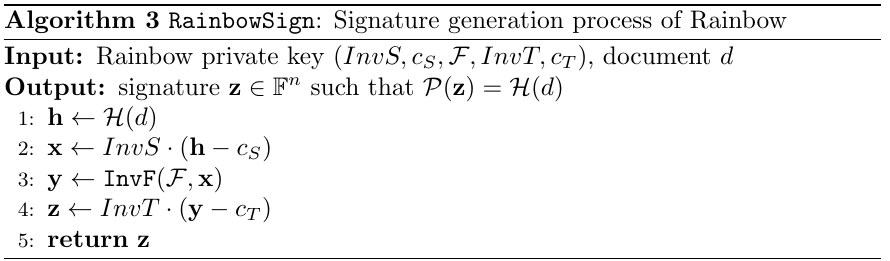
\includegraphics[width=\textwidth]{resources/rainbowsign.png}
    \caption{Pseudo code for the Rainbow signature scheme.}
    \label{rainbowsign}
\end{figure}\\
Due to the layered nature of the Rainbow scheme, the first part of \texttt{rainbow\_sign()} is used to randomly generate variables (called \emph{vinegar} variables), the linear equations of the first layer (using the \emph{vinegar} variables) while also pre-computing variables for the second \emph{rainbow layer}. Once this setup has been computed, the scheme is ready to compute line 2 in \cref{rainbowsign}.\medskip\\
As the scheme has to find a \emph{suitable} pre-image $\textbf{y} \in F$, it is not impossible to obtain a pre-image $\textbf{y}$ that is not suitable for further computation forcing the algorithm to find a new pre-image through a rerun. This is implemented as a \texttt{while}-loop running the computations of lines 2 and 3 until a point is reached where the result $\textbf{y}$ is \emph{suitable}. Such a $\textbf{y}$ would be one that allows for the system of linear equations, constructed by using the randomly generated \emph{vinegar} variables in the polynomials of $F$, to be solvable. Once the aforementioned system of linear equations is solvable $\textbf{y}$ is a suitable pre-image. The procedure can be seen in \cref{rainbowinvf}. Having computed lines 1-3 in \cref{rainbowsign}, the remaining part of the procedure is to use the pre-image $\textbf{y}$ to compute the signature $\textbf{z}$ and return that.
\begin{figure}[t]
    \centering
    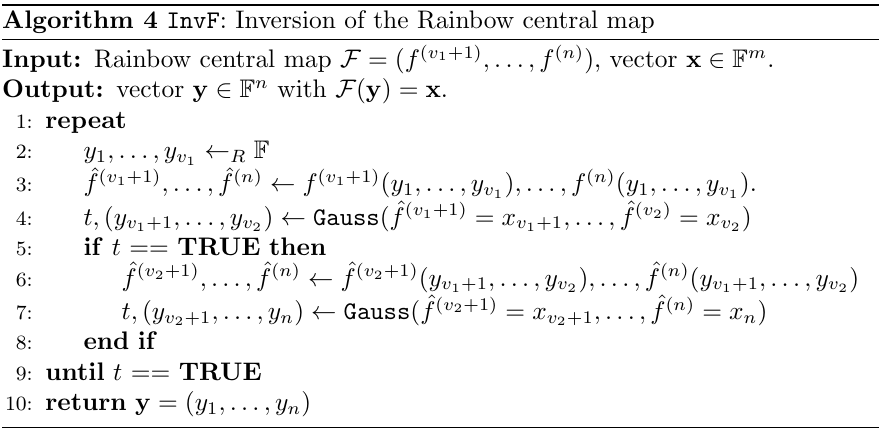
\includegraphics[width=\textwidth]{resources/rainbowinvf.png}
    \caption{Pseudo code inverting the central map $F$.}
    \label{rainbowinvf}
\end{figure}
To end off, the function \texttt{rainbow\_sign()} cleans the memory by nullifying all contents of the addresses used for the procedure.
\subsubsection{Signature Verification} \label{section:message_verif}
As the procedure in \cref{rainbowsign} uses pre-images and inverted maps to compute $\textbf{z}$, the verification procedure is quite simple. Provided a signature it can be verified by hashing the document/message in use, using the same hashing function as the signer did, and computing the public map on the given signature to then check if the values of both are the same. Figure \ref{rainbowveri} shows the pseudo code if this procedure. The procedure is, once more, ran from a \texttt{NIST}-specified function, though, this time called \texttt{crypto\_sign\_open()}. 
\begin{figure}[t]
    \centering
    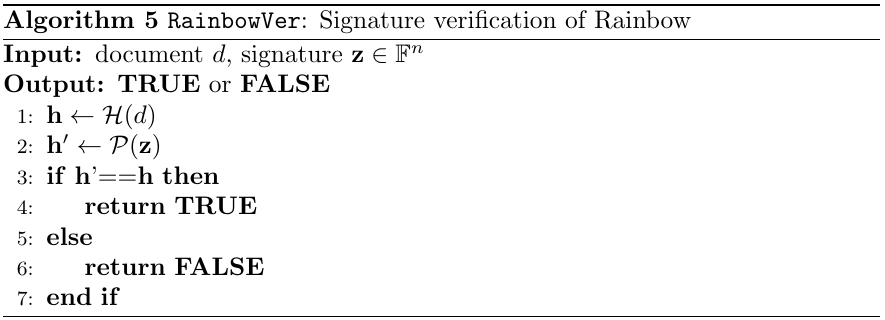
\includegraphics[width=\textwidth]{resources/rainbowver.png}
    \caption{Pseudo code for the Rainbow verification scheme.}
    \label{rainbowveri}
\end{figure}\\
For the sake of satisfactory computation, the same SHA scheme, namely SHA256, is used to compute the hash of the document $d$. Once more, the wrapper in \texttt{utils\_hash.c} is used to wrap the \texttt{RISCV-Crypto} implementation mentioned in \cref{utils}. To compute the publicmap on $\textbf{z}$, line 2 in \cref{rainbowveri}, the procedure calls \texttt{rainbow\_verify()} in \texttt{rainbow.c} to handle the remainder of the scheme.\medskip\\
The \texttt{rainbow\_verify()} function has two functionalities
\begin{enumerate}
    \item computing the publicmap using \texttt{rainbow\_publicmap()} in\\ \texttt{rainbow\_publicmap.c}, and
    \item verifying the computed publicmap against the hashed document value.
\end{enumerate}
The public map computation in \texttt{rainbow\_publicmap()} is much as one would expect for computing an output vector from a system of equations and some input the variables.\medskip\\
The actual verification is then done in \texttt{\_rainbow\_verify()} using the message digest computed by the \texttt{rainbow\_publicmap} procedure. The idea for verification checking is to check a locally hashed version of the document against the digest computed just prior. The check is a simple bit-wise \texttt{xor} for each \texttt{uint8\_t} (or just each byte) that resides in both hashes. For each byte value, the result of the bit-wise \texttt{xor} is then \texttt{or}'ed such that if the final value is larger than 0, the hashes are different and the verification returns a verification failure.

\subsubsection{Finite Field Arithmetic} \label{implementation:ffa}
%The mathematical aspect of the Rainbow scheme is quite large, as the core of the scheme is based on pure math. \textbf{NOT DONE}
As the polynomials in the public and private key maps are defined over finite fields, much of the Rainbow scheme relies on finite field arithmetic, as well as aspects of linear algebra. Performing operations like message signing requires a gaussian elimination of a linear system, as was seen in \cref{section:message_sign}. For finite field arithmetic the code uses many finite field multiplications as well as finite field additions. These arithmetic operations are not native on all platforms, and therefore are implemented through the use of non-native algorithms.\medskip\\
The linear algebra and finite field arithmetic functions are implemented in the files \texttt{gf16.h}, all files prepended with \texttt{blas} and the \texttt{parallel\_matrix\_op} files (\texttt{.c} and \texttt{.h}). The original Rainbow code relies on using Single Instruction Multiple Data (SIMD) instructions on the benchmarked platforms to obtain fast computations in the specified finite fields, $GF(256)$ and $GF(16)$ that is.
\medskip\\
The implementation of $GF(16)$ multiplications in \cite{rainbownist} relies on using \texttt{VPSHUFB/TBL} instructions for multiplication tables. Using this approach, multiple $GF(16)$ elements can be multiplied by some $GF(16)$ scalar, using the aforementioned SIMD instructions. As these instructions are native to x86 and ARM platforms, the equivalent version for RISC-V is the vector instruction set extension. For this project, as was specified in \cref{pre-riscv}, the ISA used is RV32IM meaning that the vector instructions are not available. This means that the performance between the platforms tested in \cite{rainbownist} and this RISC-V platform potentially is quite different, as the compiler is no longer able to use SIMD instructions for these computations.
\medskip\\
An alternative implementation, for time-constancy, is also given by the Rainbow authors in \cite{rainbownist}. In this version, multiplications still rely on the SIMD instructions to obtain fast multiplications for multiple elements at a time. Though, instead of using multiplication tables the new multiplication method is using logarithm and exponentiation tables such that $a \cdot b = g^{(\log_g a +  \log_g b)}$ with $\log_g 0 = -42$ \cite{rainbownist}.
\medskip\\
The functions implementing the aforementioned functionality are used as subprocedures for the general public key evaluation method given by Tung Chou, as mentioned in \cite{rainbownist}. The specifics of this general method will not be gone through in this report. Intead, having focus on the finite field operations done by the Rainbow reference implementation, the functionality mentioned in the former paragraphs have been implemented in \texttt{blas\_u32.h}, \texttt{gf16.h} and \texttt{blas.h}. Specifically for Rainbow level I, the multiplication scheme used when evaluating the \texttt{GF(16)} coefficients of the multivariate polynomials against their corresponding monomials is done in \texttt{blas\_u32.h} using the \texttt{\_gf16v\_mul\_scalar\_u32()} function (being aliased \texttt{blas.h} to \texttt{gf16v\_mul\_scalar()}.
\medskip\\
Using Rainbow level III and V will require additional computations as the elements are over $GF(256)$ instead of $GF(16)$. These computations can either be done using the same SIMD instruction principles as was done for $GF(16)$ or using the Karatsuba algorithm to obtain a fast multiplication of elements. The latter of which uses the same representation as I did for the optimizations mentioned in \cref{opti}. Although these security levels were not in focus during this project, the reference functionality for them is still available such that any future optimization is easily available.
\subsection{Testing Environment}
As all aforementioned functionality was implemented and ran on a simulated device that does not interact with the host machine operating system in the same way that a typical program would, the testing facilities also had to be a little different. It therefore seems reasonable to shortly discuss how all aforementioned functionality was tested, as any errors in testing usually is quite a bad sign later in the pipeline. The primary file used for testing is the \texttt{kat.py} file in the \texttt{test/} directory.\medskip\\
First of all, to be able to test the scheme the host device and the client device had to be able to communicate. Usually this can be done via some sort of serial port on an actual device, though as this was a virtual device a serial port was not present. The author(s) of the \texttt{pqriscv} project ensured there to be a runtime option that allows for the client device to have a communications port through a linux \texttt{pts} device.\medskip\\
Before any actual communication between client and \texttt{kat.py}, the \texttt{kat.py} script will run some preparations to ensure that it is ready to check for correct outputs from the client device. For \texttt{kat.py} to check correctness it has access to a host-native Rainbow implementation, directly pulled from the github submission repository, which it then compiles and runs before any testing on the client device. This means that before any test, the \texttt{kat.py} file will generate a \texttt{KAT\_<timestamp>} folder that holds the randomseed used, the keys generated from the random seed, the message, an incorrect signature (although this is generated, it is not of importance for the current state of the test-suite) and the signature generated given the keys and message in the folder. This collection of files constitutes a \textit{Known Answer Test} or KAT and is used by the \texttt{kat.py} script to check for correctness in the implementation.\medskip\\
The initial communication between the test-suite and the client device has the test-suite send all required items to the client device. When key-generation is tested, the input is just the random seed needed for the client device to generate a keypair. For signing and verification the test-script will send the message, a key (public for verification and private for signing) and a signature, being of course only for verification. Once these values have been provided, the script will wait for the client device to answer. For key generation the script checks if the byte-values of the host-native scheme are equal to the byte values of the client scheme. For signing, only signature byte-values are checked, while verification checks for any inconsistencies in the \texttt{true}/\texttt{false} output of the client, still compared to the host-native version.
\medskip\\
The testing script is also accompanied by a shell-script, called \texttt{multitest.sh}, for running multiple tests or benchmarks on the different implementations and saving the results in the corresponding \texttt{KAT} folder. Using the output of potential benchmark runs (after running \texttt{multitest.sh}), the \texttt{grapher.py} script allows for easy bar-plotting of key aspects for evaluation.